% Define block styles
\tikzstyle{block} = [draw, rectangle, text centered, text width=10em, minimum height=0.5em, rounded corners=true]
\tikzstyle{arrowtext} = [text width=4em, text centered]
\tikzstyle{arrow} = [draw, -latex]

\definecolor{red1}{RGB}{160,0,0}
\definecolor{green1}{RGB}{0,160,0}
\definecolor{blue1}{RGB}{0,0,160}
\definecolor{black}{RGB}{0,0,0}
\definecolor{white}{RGB}{255,255,255}

\usetikzlibrary{shapes.geometric,arrows,positioning}

	      
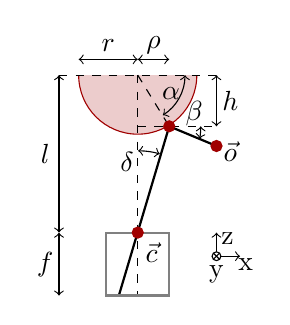
\begin{tikzpicture}[node distance=4em, auto]
    % circle
    \draw[red1, fill=red1!20] (-0.75,0) arc (-180:0:0.75);

	\coordinate (m) at (0.4,-0.65);
	\coordinate (mm) at (0.8,-1.3);
	\coordinate (o) at (1.0,-0.9);
	\coordinate (c) at (  0,-2.0);

    \draw [-, dashed] (0,0) |- (0,-2.8);       % Line of sight
    \draw [-, dashed] (-1,0) |- (1,0);         % Upper end of b, h
    \draw [-, dashed] (0,-0.65) |- (1,-0.65);  % Lower end of h
    \draw [-, dashed] (0,0) -- (m);            % Line of reflection
    % \draw [-, dashed] (0,0) -- (mm);         % Extension

    % Mini-Coordinate-System
    \draw [->] (1.0,-2.3) |- (1.3,-2.3) node [xshift=0.2em,yshift=-0.3em,anchor=center] {x};
    \draw [->] (1.0,-2.3) -- (1.0,-2.0) node [xshift=0.4em,yshift=-0.2em,anchor=center] {z};
    \draw [color=black, fill=white] (1.0,-2.3) circle(0.056) node [below] {y};
    \draw [-] (0.96,-2.34) -- (1.04,-2.26);
    \draw [-] (0.96,-2.26) -- (1.04,-2.34);

    % Light
    \draw[-, thick] (m) -- (-0.24,-2.8);
    \draw[-, thick] (m) -- (o);

    % camera
    %\draw [-, thick, gray] (-0.5,-2)
    %    -- (0.5,-2)
    %    -- (0.3,-2.3)
    %    -- (-0.3,-2.3)
    %    -- (-0.5,-2);
    \draw [-, thick, gray] (0.4,-2.0) 
        -- (0.4,-2.8)
        -- (-0.4,-2.8)
        -- (-0.4,-2.0)
        -- cycle;

    % points
    %\draw[fill=red1, color=red1] (0,0) circle (2pt) node [below, color=black, xshift=-0.5em] {$\vec{c}$};
    \draw[fill=red1, color=red1] (m) circle (2pt) node [below, color=black, xshift=0.25em] {}; % was: $\hat{\vec o}$
    \draw[fill=red1, color=red1] (o) circle (2pt) node [below, color=black, xshift=0.5em, yshift=0.5em] {$\vec o$};
    \draw[fill=red1, color=red1] (c) circle (2pt) node [below, color=black, xshift=0.5em] {$\vec c$};

    % sizes
    \path[<->]
        (-1.0,0) edge node [xshift=-0.5em, anchor=center] {$l$} (-1.0,-2.0)
        (-1.0,-2.0) edge node [xshift=-0.5em, anchor=center] {$f$} (-1.0,-2.8)
        %(0.0,0.0) edge node [xshift=-0.5em, anchor=center] {$r$} (0.0,-0.75)
        (1.0,0.0) edge node [xshift=0.5em, anchor=center] {$h$} (1.0,-0.65)
        (0.0,0.2) edge node [yshift=0.5em, anchor=center] {$\rho$} (0.4,0.2)
        (0.0,0.2) edge node [yshift=0.5em, anchor=center] {$r$} (-0.75,0.2);

    % angles
        \draw[black, fill=none, <->] (0.6,0.0) arc (0:-58:0.6) node [xshift=0.3em, yshift=0.8em] {$\alpha$};
        \draw[black, fill=none, <->] (0.8,-0.65) arc (0:-9:1) node [xshift=-0.2em, yshift=0.9em] {$\beta$};
        %\draw[black, fill=none, <->] (0.2,-0.9) arc (65:90:0.5) node [xshift=-0.4em, yshift=-0.4em] {$\delta$};
        \draw[black, fill=none, <->] (0.28,-1) arc (74:90:1) node [xshift=-0.4em, yshift=-0.4em] {$\delta$};
\end{tikzpicture}
